\documentclass[tikz,border=6pt]{standalone}
\usepackage{tikz}
\usepackage{amsmath}
\usetikzlibrary{arrows.meta,calc,positioning,shapes.geometric,shapes.misc,
                backgrounds,fit,decorations.pathmorphing}

\begin{document}
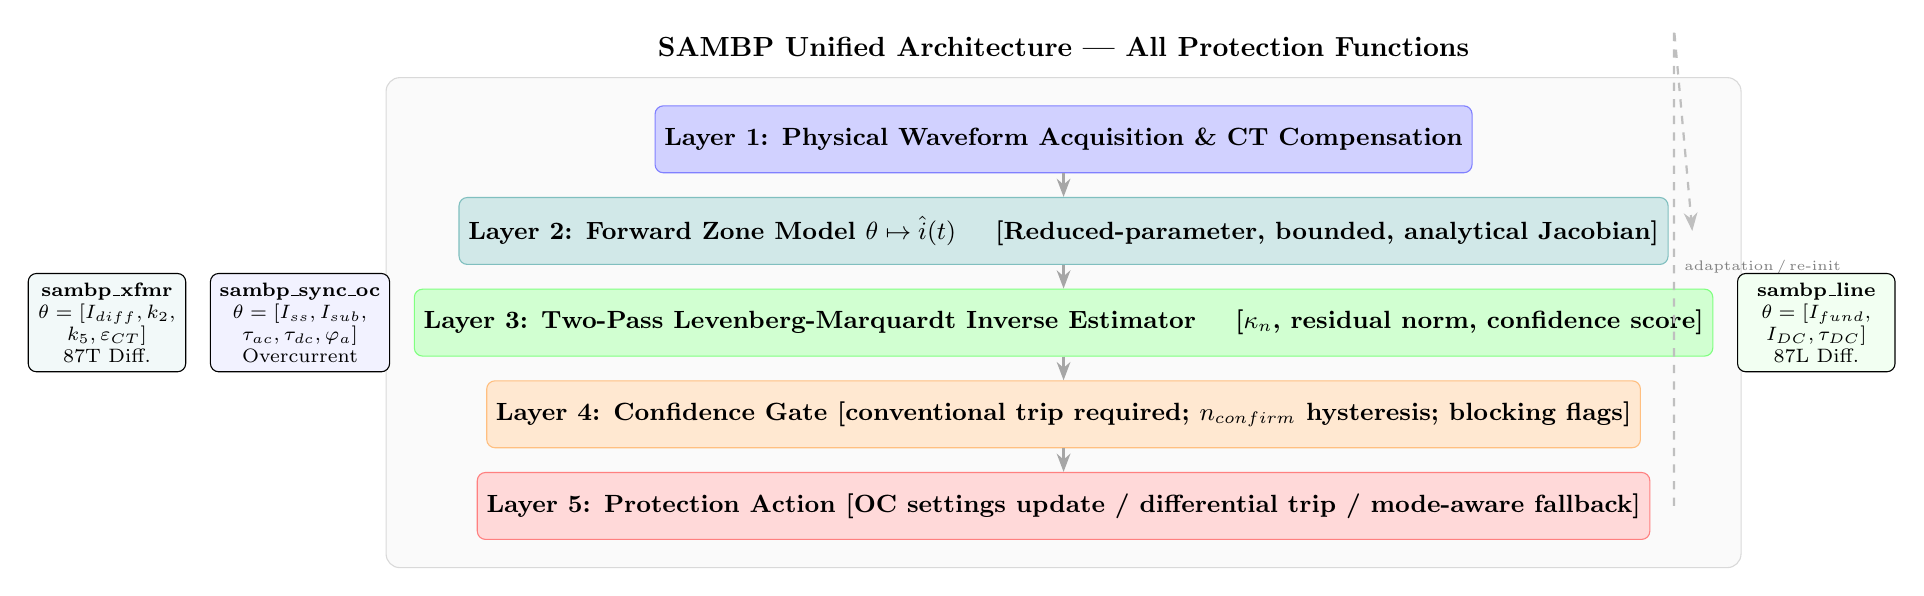
\begin{tikzpicture}[
  font=\small,
  >=Stealth,
  layer/.style  ={draw,rectangle,minimum width=9.5cm,minimum height=0.85cm,
                  align=center,font=\small\bfseries,rounded corners=3pt},
  L1/.style={layer,fill=blue!18,draw=blue!50},
  L2/.style={layer,fill=teal!18,draw=teal!50},
  L3/.style={layer,fill=green!18,draw=green!50},
  L4/.style={layer,fill=orange!18,draw=orange!50},
  L5/.style={layer,fill=red!15,draw=red!50},
  arrow/.style={->,thick,gray!70},
  annot/.style ={draw,fill=white,rounded corners=2pt,
                 font=\scriptsize,align=left,inner sep=4pt},
]

%% ===== Title =================================================================
\node[font=\normalsize\bfseries] (title) at (0,0)
      {SAMBP Unified Architecture — All Protection Functions};

%% ===== Layers ================================================================
\node[L1,below=0.5cm of title]  (l1)
      {Layer 1: Physical Waveform Acquisition \& CT Compensation};
\node[L2,below=0.3cm of l1]     (l2)
      {Layer 2: Forward Zone Model  $\theta \mapsto \hat{i}(t)$
       \hspace{1em}[Reduced-parameter, bounded, analytical Jacobian]};
\node[L3,below=0.3cm of l2]     (l3)
      {Layer 3: Two-Pass Levenberg-Marquardt Inverse Estimator
       \hspace{1em}[$\kappa_n$, residual norm, confidence score]};
\node[L4,below=0.3cm of l3]     (l4)
      {Layer 4: Confidence Gate  [conventional trip required;
       $n_{confirm}$ hysteresis; blocking flags]};
\node[L5,below=0.3cm of l4]     (l5)
      {Layer 5: Protection Action  [OC settings update / differential trip /
       mode-aware fallback]};

%% ===== Arrows between layers =================================================
\foreach \a/\b in {l1/l2, l2/l3, l3/l4, l4/l5} {
  \draw[arrow] (\a.south) -- (\b.north);
}

%% ===== Vertical dashed feedback arrow =======================================
\draw[->,thick,dashed,gray!50]
      ($(l5.east)+(0.3,0)$) -- ($(l5.east)+(0.3,0)+(0,3.2*0.3+4*1.15+0.5)$)
      node[midway,right,font=\tiny,gray]{adaptation\,/\,re-init}
      -- ($(l2.east)+(0.3,0)$);

%% ===== Project column labels =================================================
\node[font=\scriptsize\bfseries,blue!60!black] (pA)
      at (-6.2,0) {};

\node[draw,fill=blue!5,rounded corners=3pt,
      left=0.3cm of l3,font=\scriptsize,align=center,
      minimum width=2.0cm] (oc)
      {\textbf{sambp\_sync\_oc}\\
       $\theta=[I_{ss},I_{sub},$\\$\tau_{ac},\tau_{dc},\varphi_a]$\\
       Overcurrent};

\node[draw,fill=teal!5,rounded corners=3pt,
      left=0.3cm of oc,font=\scriptsize,align=center,
      minimum width=2.0cm] (t87)
      {\textbf{sambp\_xfmr}\\
       $\theta=[I_{diff},k_2,$\\$k_5,\varepsilon_{CT}]$\\
       87T Diff.};

\node[draw,fill=green!5,rounded corners=3pt,
      right=0.3cm of l3,font=\scriptsize,align=center,
      minimum width=2.0cm] (l87)
      {\textbf{sambp\_line}\\
       $\theta=[I_{fund},$\\$I_{DC},\tau_{DC}]$\\
       87L Diff.};

\begin{scope}[on background layer]
  \node[draw=gray!30,fill=gray!4,rounded corners=5pt,
        fit=(l1)(l2)(l3)(l4)(l5),inner sep=10pt] {};
\end{scope}

\end{tikzpicture}
\end{document}
